\documentclass{article}
\usepackage[utf8]{inputenc}
\usepackage[margin=1in]{geometry}

\usepackage{graphicx}
\usepackage{wrapfig}
\usepackage{verbatim}
\usepackage{enumitem}

\title{Line Sweep and Convex Hull}
\author{Kevin Geng\footnote{Thanks to information on TopCoder and lectures created by Alex Chen and Hariank Muthakana.}}
\date{16 December 2016}


\begin{document}

\maketitle

%\section{Introduction}
%Computational Geometry is a category of problems that is exactly what it sounds like. Make a computer do geometry for you!

\section{Intersecting line segments}


\begin{wrapfigure}{r}{0.3\textwidth}
  \vspace{-30pt}
  \begin{center}
    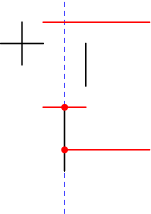
\includegraphics[width=0.20\textwidth]{linesvh.png}
  \end{center}
  \vspace{-10pt}
  \caption{An example of a sweep line. \textit{Credit: TopCoder.}}
  \vspace{-20pt}
\end{wrapfigure}

Suppose we have $N$ horizontal and vertical line segments. How can we find all points at which two of these intersect? One solution is to look at every pair of horizontal and vertical line segments, and determine whether they intersect by checking that the x coordinate of the vertical line falls within the horizontal line, and vice versa. This solution is $O(N^2)$.

However, we can do better by using a line sweep algorithm. Conceptually, imagine a line sweeping from left to right across the xy-plane. We will examine the line at certain x-coordinates we are interested in. We can think of these as \textit{events} which we sort in order of increasing x-coordinate. For this problem, we are interested in:

\begin{enumerate}
    \itemsep 0em
    \item A vertical segment
    \item The start of a horizontal segment
    \item The end of a horizontal segment
\end{enumerate}

The key to line sweep is to have the sweep line hold information. We will keep an \textit{active set} describing what horizontal segment are currently intersected by the sweep line. Whenever we encounter the start or end of a horizontal segment, we will add or remove it from the set. To implement this active set, we can use a binary search tree, and sort the horizontal segments by their y-coordinate.

Now, whenever we encounter a vertical line, we simply examine our active set. In the range of y-coordinates that the vertical line spans, is the sweep line currently intersecting any horizontal lines? If so, we have an intersection! Each insertion and deletion takes $O(log N)$. If we need to keep track of insertions, the total complexity is $O(N log N + I)$.

\subsection{More problems}

\begin{itemize}
    \item Solve the intersecting line segments problem, but for lines that are not necessarily horizontal or vertical.
    \item Given $N$ points in two-dimensional space, find the two points that are closest together.

    \item USACO 2013 November, Silver Problem 2: Crowded Cows
    
    Farmer John's N cows ($1 \leq N \leq 50,000$) are grazing along a one-dimensional fence.  Cow $i$ is standing at location $x(i)$ and has height $h(i)$ ($1 \leq x(i), h(i) \leq 1,000,000,000$).  

    A cow feels "crowded" if there is another cow at least twice her height within distance D on her left, and also another cow at least twice her height within distance D on her right ($1 \leq D \leq 1,000,000,000$).  Since crowded cows produce less milk, Farmer John would like to count the number of such cows.  Please help him.
    
    \item USACO 2013 February, Silver Problem 2: Square Overlap
    \item USACO 2012 February, Silver Problem 1: Overplanting
\end{itemize}


\begin{comment}
\section{Line sweep with segment trees}

Hello, world.

\begin{itemize}[leftmargin=*]
    \item[] USACO 2016 January, Platinum Problem 2: Mowing the Field

    Farmer John is quite reliable in all aspects of managing his farm, except one: he is terrible at mowing the grass in a timely fashion. He only manages to move the mowing machine once per day, in fact. On day $1$, he starts at position $(x_1, y_1)$ and on day $d$ he mows along a straight segment to the position $(x_d, y_d)$, moving either horizontally or vertically on the 2D map of his farm; that is, either $x_d = x_{d-1}$, or $y_d = y_{d-1}$. FJ alternates between horizontal and vertical moves on successive days.

So slow is FJ's progress that some of the grass he mows might grow back before he is finished with all his mowing. Any section of grass that is cut in day $d$ will reappear on day $d+T$, so if FJ's mowing path crosses a path he cut at least $T$ days earlier, he will end up cutting grass at the same point again. In an effort to try and reform his poor mowing strategy, FJ would like to count the number of times this happens.

Please count the number of times FJ's mowing path crosses over an earlier segment on which grass has already grown back. You should only count "perpendicular" crossings, defined as a point in common between a horizontal and a vertical segment that is an endpoint of neither.
\end{itemize}
\end{comment}

\section{Convex hull}

\begin{wrapfigure}{r}{0.3\textwidth}
  \vspace{-40pt}
  \begin{center}
    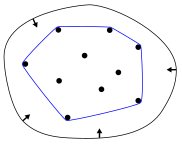
\includegraphics[width=0.25\textwidth]{ConvexHull.png}
  \end{center}
  \vspace{-10pt}
  \caption{Analogy between a convex hull and an elastic band. \textit{Credit: Wikipedia.}}
  \vspace{-20pt}
\end{wrapfigure}

The convex hull of a set of points is the smallest convex polygon that can enclose all of them. One way to visualize this is to think of the points as pins, then imagine wrapping a rubber band around them.

\subsection{Gift wrapping}

This is the simplest way to find the convex hull. We start at the leftmost point in the set, $p_0$. At each step $i$, we find the angle from $p_i$ to every other point, and pick $p_{i+1}$ so that all points lie to the right of the line segment between $p_{i-1}$ and $p_i$. We continue until we reach the original point. Since we examine $n$ points for each of $h$ elements in the convex hull, the complexity is $O(nh)$.

\subsection{Graham scan}



We can solve the convex hull problem using the \textit{Graham scan} algorithm, which functions similar to a line sweep. First, we pick an "origin" point to start from, perhaps the one with the lowest y-coordinate. Then, we find the angles from that point to all other points, and sort the points in counterclockwise order.

Then we iterate through the points in that order. For each point $p_i$, we examine the angle it forms with the previous two points, $\angle p_i p_{i-1} p_{i-2}$. If the angle would result in a concave polygon, we delete $p_{i-1}$ and check again. We can check this quickly by performing a cross product and examining its sign.

The initial sort has a complexity of $O(N log N)$. The actual loop only has a complexity of $O(N)$, because each point is checked at most twice. So the overall complexity is $O(N log N)$.

\begin{figure}[h]
  \centering
  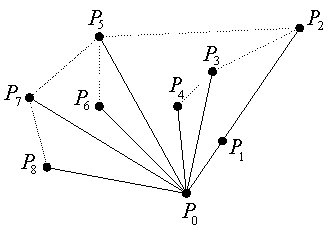
\includegraphics[width=0.4\textwidth]{Pic_graham2.jpg}
  \caption{Representation of Graham scan algorithm. \textit{Credit: geomalgorithms.com}}
\end{figure}

\begin{comment}
\section{Computational Geometry Toolkit}

\subsection{Dot Product}
Suppose we want to find the distance from a point $p$ to a line $l$ described by two points $a$ and $b$. (Hint: We learned about this in Multi.) The shortest line from $p$ to $l$ is the one that is perpendicular to $l$. Therefore, the length of this line is equal to the dot product of the unit vector normal to $l$ and the vector from $p$ to $a$ (or from $p$ to $b$).

\subsection{Cross Product}


\subsection{Shoelace}

\subsection{Angles}

\subsection{Distances}
\end{comment}
\end{document}
